%%%%%%%%%%%%%%%%%%%%%%%%%%%%%%%%%%%%%%%%%%%%%%%%%%%%%%%%%%%%%%%%%%%%%%%%
% Preamble
%%%%%%%%%%%%%%%%%%%%%%%%%%%%%%%%%%%%%%%%%%%%%%%%%%%%%%%%%%%%%%%%%%%%%%%%
\documentclass[11pt]{article}
%
% Packages and other includes
% Pagination
\usepackage[letterpaper, margin=1.25in]{geometry}
%
% Graphics, floats, tables
\usepackage{graphicx, color, float, array}
%
% Hyperlinks
\usepackage{hyperref}
%
% AMS packages for equations, math symbols
\usepackage{amsmath, amssymb, braket}
%
% Bibliography
\usepackage[style=numeric,sorting=none]{biblatex}
\addbibresource{referencesProject4.bib}
%
% Revision (see Makefile)
\newcommand{\Revision}{977be36}

%
% Definitions and settings
% Paragraph indent and spacing
\setlength{\parskip}{0.4\baselineskip}
\setlength{\parindent}{0in}
%
% Math mode version of "r" column type (requires array package)
\newcolumntype{R}{>{$}r<{$}}
%
% Title, authors, date
\title{\textbf{Bimetallic Metallocene Hydrides}}
\author{Brian Nguyen and Luke Nambi}
\date{Chem 150L Winter 2018 \\ \today, Revision \Revision}

\newcommand*{\comment}[1]{{\color{blue} #1}}
%
%
%%%%%%%%%%%%%%%%%%%%%%%%%%%%%%%%%%%%%%%%%%%%%%%%%%%%%%%%%%%%%%%%%%%%%%%%
% Main document
%%%%%%%%%%%%%%%%%%%%%%%%%%%%%%%%%%%%%%%%%%%%%%%%%%%%%%%%%%%%%%%%%%%%%%%%
%
\begin{document}

\maketitle

\begin{abstract}

  \noindent Recent studies have reported the synthesis of precusors
  for or 4f$^n$5d$^1$ Ln$^{2+}$ ions that could form 5d$^1$5d$^1$
  metal - metal bonded complexes. The electronic structure of [(Cp)$_2$Y($\mu$-H)]$_2$
  and [(Cp)$_2$Y($\mu$-H)]$^-_2$ (see Fig. 1) are investigated for metal-metal bonding.
  This investigation uses the natural orbitals from a Kohn-Sham
  Density Functional Theory geometry optimization calculation, 
  validated by comparison to geometry data from the literature. 
  The singly occupied molecular orbital of the anion is $\sigma$-bonding
  between the two metal centers, hence there is metal-metal
  bonding of order 0.5 for the anion and no metal-metal bonding
  for the neutral complex.
\end{abstract}


\begin{figure}[htbp]
  \centering
  \label{fig:YYchemStruct}

  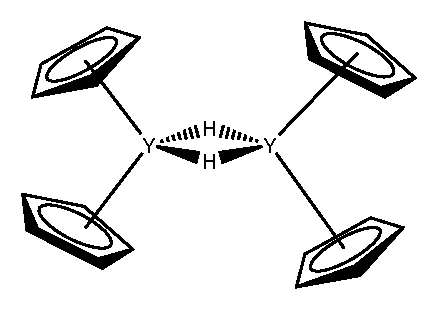
\includegraphics[width=.40\textwidth]{neutral.eps}
  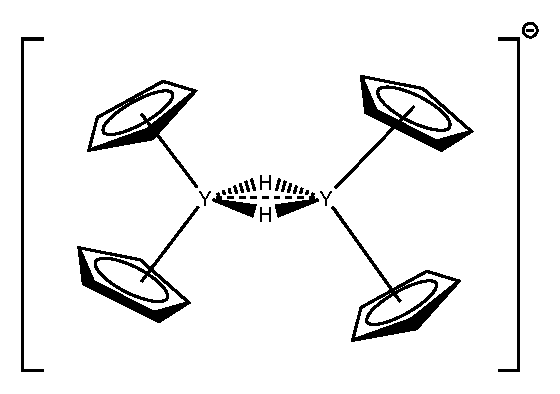
\includegraphics[width=.49\textwidth]{anion.eps}

  \caption{Chemical structure of [(Cp)$_2$Y($\mu$-H)]$_2$ (left)
  and [(Cp)$_2$Y($\mu$-H)]$^-_2$ (right)}
\end{figure}

\section{Introduction}
Unusual oxidation states have played important roles in redox chemistry.
The investigations of the divalent lanthanide e.g. SmI$_2$ have led to
unexpected discoveries that had broad applications in organic and
organometallic synthesis. Divalent lanthanides are of great interest
to open up new options in reductive chemistry. This requires an understanding
of these cationic states. Under special ligand environment, divalent lanthanides
are stabilized and we hypothesize that the stability is attributed to the
metal-metal bond in the bimetallic rare-earth complex.

Lanthanide elements are chemically similar with slightly different radial
size that gradually changes between 0.01 and 0.02 $\AA$  from element to element.
This unique property may potentially provide avenues to optimize the chemistry
in ways not possible for other series of metals in the periodic table where
one would typically optimize the ligand set.

%The first paragraph of the introduction should explain the broader
%context of the computational experiment (1-2 sentences) and then
%funnel the reader towards the research hypothesis/question posed in the
%lab assignment.
%
%In the second paragraph any relevant existing work in the literature should
%be referenced, and the relation of this work to the current paper needs
%to be stated and explained. An original research paper needs to present
%something new and significant, and explain how its content goes beyond
%existing work; for a lab report this paragraph can just state key
%references and sources.

\section{Methods}

\subsection{Statement of the Models}

Kohn-Sham Density Functional Theory(KS-DFT) is known to produce
reasonable electronic structure for molecules, and has been
widely applied. The energy($E$) of a molecular system is a functional
of the non-interacting KS-orbitals($\Phi^{KS}$), which are constrained to 
generate the electron density of the real system:

\begin{equation}
  \label{eq:KSDFT}
  E[\rho(\Phi^{KS})] = T_s[\Phi^{KS}] + U[\rho(\Phi^{KS})] +\
  E_{xc}[\rho(\Phi^{KS})] + V[\rho(\Phi^{KS})].
\end{equation}

As non-interacting orbitals that give the correct density for the
system, the natural KS-orbitals squared give 
one of the best representations of
the reduced one-particle density for each electron.
These natural orbitals can be used to analyse the bonding in the
system.

KS-DFT is approximate due to the unknown form of $E_{xc}$, the
exchange correlation functional. Recently, meta-GGA hybrids have
been developed that are a reasonable approximation to the exact
exchange correlation - the TPSSh functional is further described
in the computational details.

To obtain a rough picture of the bonding, a relatively small split
valence basis set can be used that balances basis set
incompleteness and basis set superposition. The choice of basis
is described in the computational section.


\subsection{Computational Details}

The geometry optimization calculations for all molecules was
performed with {\sc Turbomole} 7.2\cite{TURBOMOLE} , 
using the TPSS-h meta-GGA hybrid
functional\cite{Tao.J:PRL.2003}
with the def2-SVP basis set \cite{Weigend.F:PCCP.2005}. 
Grimme's D3 dispersion corrections
\cite{JCC:JCC20495,doi:10.1063/1.3382344}
were turned on, as well as the RI approximation to speed up the
calculations. An effective core potential for Y was used
\cite{Andrae.D:TCA.1990}
The default threshold of
1E-7 for electronic structure convergence (\$scfconv) and 1E-3
for geometry convergence (-gcart) were used, with a gridsize of m5 
for numerical integration.\cite{Treutler95a}

For the calculations with solvent correction, the perimittivity
of the solvent was set to 7.600, and the radii for the solvent
was set to 1.30.\cite{COSMO}  All other values were their default. These
parameters correspond to THF. (Question 4.1.1)

After convergence, natural orbitals were
calculated and visualised from .cub files using ``ridft -proper"
and the vmd program. Contour values of 0.03 magnitude were used.
Localized orbitals were not computed as the natural KS-orbitals are
a better reflection of eigenstates of the electrons.

The script ``tm2molden" was used to transform the output into the
molden format. Molden 4.6 was used to measure the bond lengths.

\section{Results}

\subsection{Spin-state of molecule}

The neutral molecule can be partitioned into ionic ligands
around a cation(see Fig. \ref{fig:chargePartition}). 
Doing so identifies the cation as
Yittrium(III). Y$^{3+}$ has the electronic configuration of Kr,
with no unpaired electrons. The ligands are all also closed
shell. Therefore the neutral molecule should be closed shell
with no unpaired electrons - and therefore dimagnetic and not
active in EPR(Question 4.1.3a). 
This electronic configuration is fed into the
calculation.

The anion can be partitioned with either both Yittrium with
oxidation state 2.5 or one Yittrium(III) and one Yittrium(II).
Either result gives a complex in the doublet state, with one
unpaired electron. This is a paramagnetic electron configuration
which is active in EPR(Question 4.1.3b). 
This electronic configuration is fed into the calculation.

\begin{figure}[htbp]
  \centering

  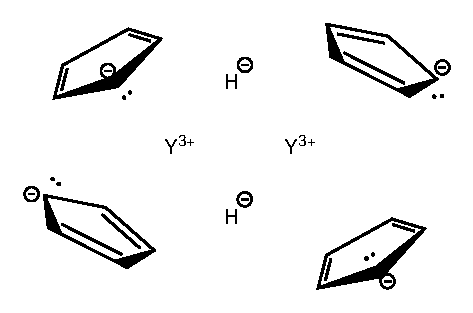
\includegraphics[width=.40\textwidth]{ionicCFtheory.eps}

  \caption{Partitioning charges in the neutral molecule}
  \label{fig:chargePartition}
\end{figure}

\subsection{Metal-metal Distance}

The optimized geometry from the calculations is compared to the
literature in Table 1.(Question 4.1.2)

\begin{table}[H]
\label{tab:atom2atomDistance}
\begin{tabular}{|ccc|RR|RR|}
  \hline
  Molecule & Atoms & Environment & \multicolumn{2}{c|}{Calc. Distance} 
  & \multicolumn{2}{c|}{Lit. Distance} \\
  &&& Angstroms & a.u. &Angstroms& a.u.\\
  \hline
  \hline
  [(Cp)$_2$Y($\mu$-H)]$_2$&Y-Y&gas-phase&3.47388&6.56469&& \\
  \hline
  [(Cp)$_2$Y($\mu$-H)]$_2$&Y-Y&Cosmo-THF&3.47468&6.56619&& \\
  \hline
  [(Cp')$_2$Y(THF)]$_2$($\mu$-O)&Y-Y&crystal&&&4.09&7.73 \\
  \hline
  [(Cp)$_2$Y($\mu$-H)]$^-_2$&Y-Y&gas-phase&3.47443&6.56572&& \\
  \hline
  [(Cp)$_2$Y($\mu$-H)]$^-_2$&Y-Y&Cosmo-THF&3.47443&6.56572&& \\
%  \hline
%  [(Cp)$_2$Y($\mu$-H)]$^-_2$&Y-Y&crystal&&&4.09&7.73 \\
  \hline
  B$_2$H$_6$&B-B&gas-phase&1.74954&3.30615&& \\
  \hline
\end{tabular}

\caption{Interatomic distances between the two centers bridged
by hydrides: Comparing calculated and literature data. Cp'= (C$_5$H$_4$SiMe$_3$)$^{1−}$} 
\end{table}

For both neutral and anion Yttrium complexes,the bond distances
in gas phase and in solvent are similar. In this report, we will
only look at the solvated structures.
%The anion has an insignificant difference in the distance
%between the metal centers.

\subsection{Natural Molecular Orbitals}

The visualization of the frontier orbitals allows for the
analysis of the bond orders in the molecules.

The neutral molecule shows bonding with the hydrides,
similar to B$_2$H$_6$. There is no metal-metal bonding in the
neutral molecule.

\begin{figure}[H]
  \centering
  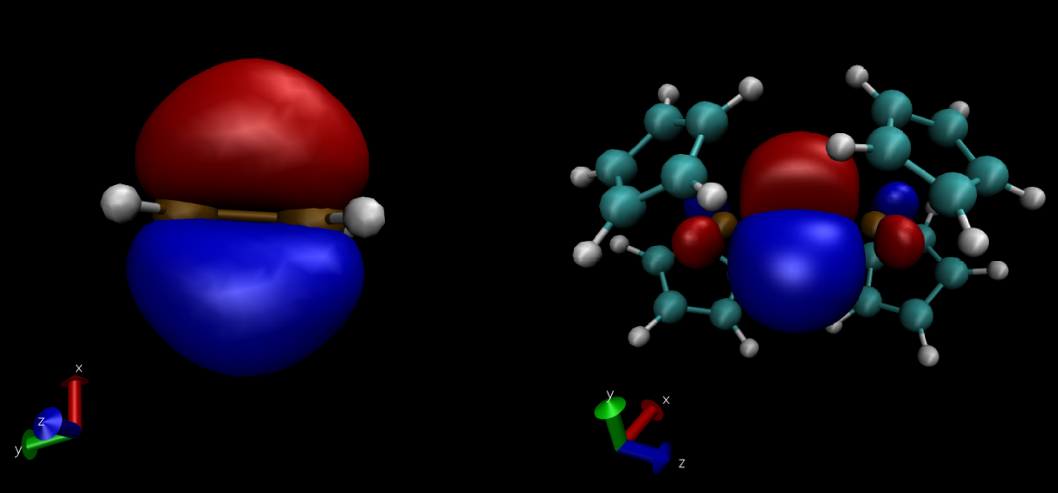
\includegraphics[scale=0.2]{b2h6_ytt.png}
  \caption{This is a sigma bond between the p-orbital of the borane
    and the s-orbital of the hydride in diborane (HOMO$-$3) (left) compared
    to the sigma bond between the d-orbital of Yttrium and s-orbital of the hydride in neutral
    bimetallic Yttrium complex (HOMO$-$8) (right).}
  \label{fig:hydride}
\end{figure}

\begin{figure}[htbp]
  \centering
  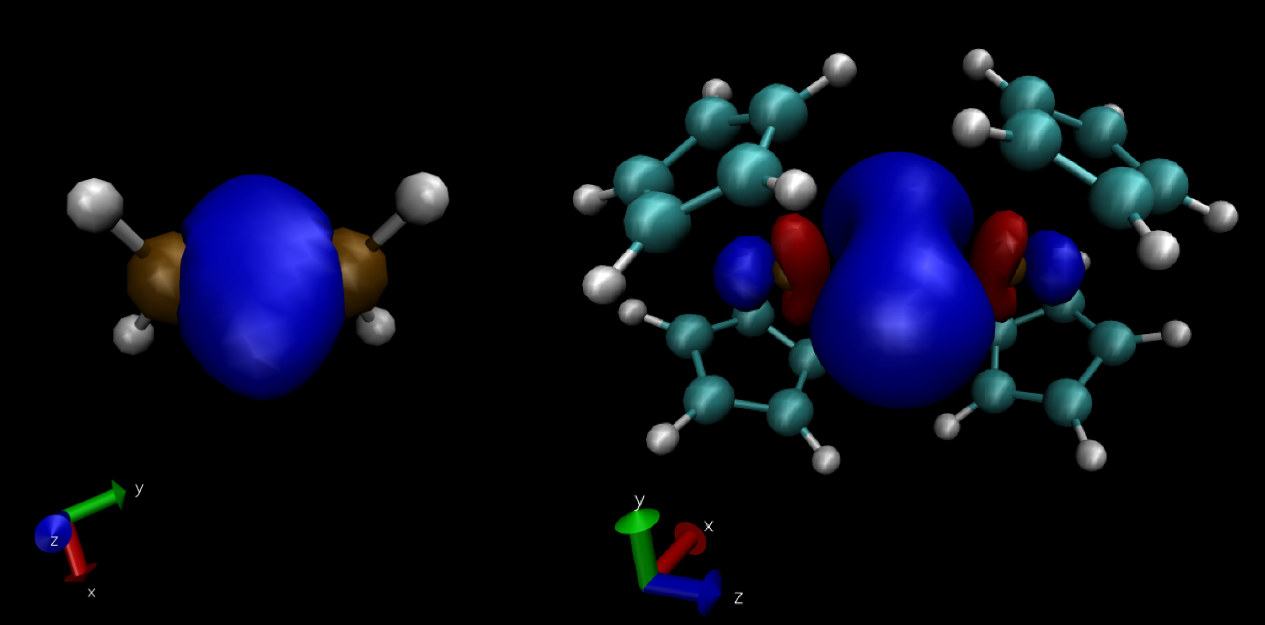
\includegraphics[scale=0.2]{hhbond.png}
  \caption{This is a sigma bond between the hydride for the diborane (HOMO$-$5) (left)
  and the neutral bimetallic Yttrium complex (HOMO$-$9) (right).
    The contour value for diborane is set to
    0.1 to emphasize the sigma bond between the hydrides since all the hydrogens participate in
    this orbital.}
  \label{fig:hhbond}
\end{figure}

In comparison to the work by Dumas et al\cite{DUMAS201738}, there is no participation of
the Yttrium d-orbitals in this bond and instead there is slight anti-bonding with the
p-orbitals of Yttrium. This may be due to the smaller def2-SVP basis set used in this
calculation.
%\comment{insert hydride bonds of neutral complex and B2H6 here}

The information above can be used to create a minimal molecular orbital diagram
for both the neutral molecule and B$_2$H$_6$ in Fig \ref{fig:minimal}.(Question 4.1.5)

\begin{figure}[H]
  \centering
  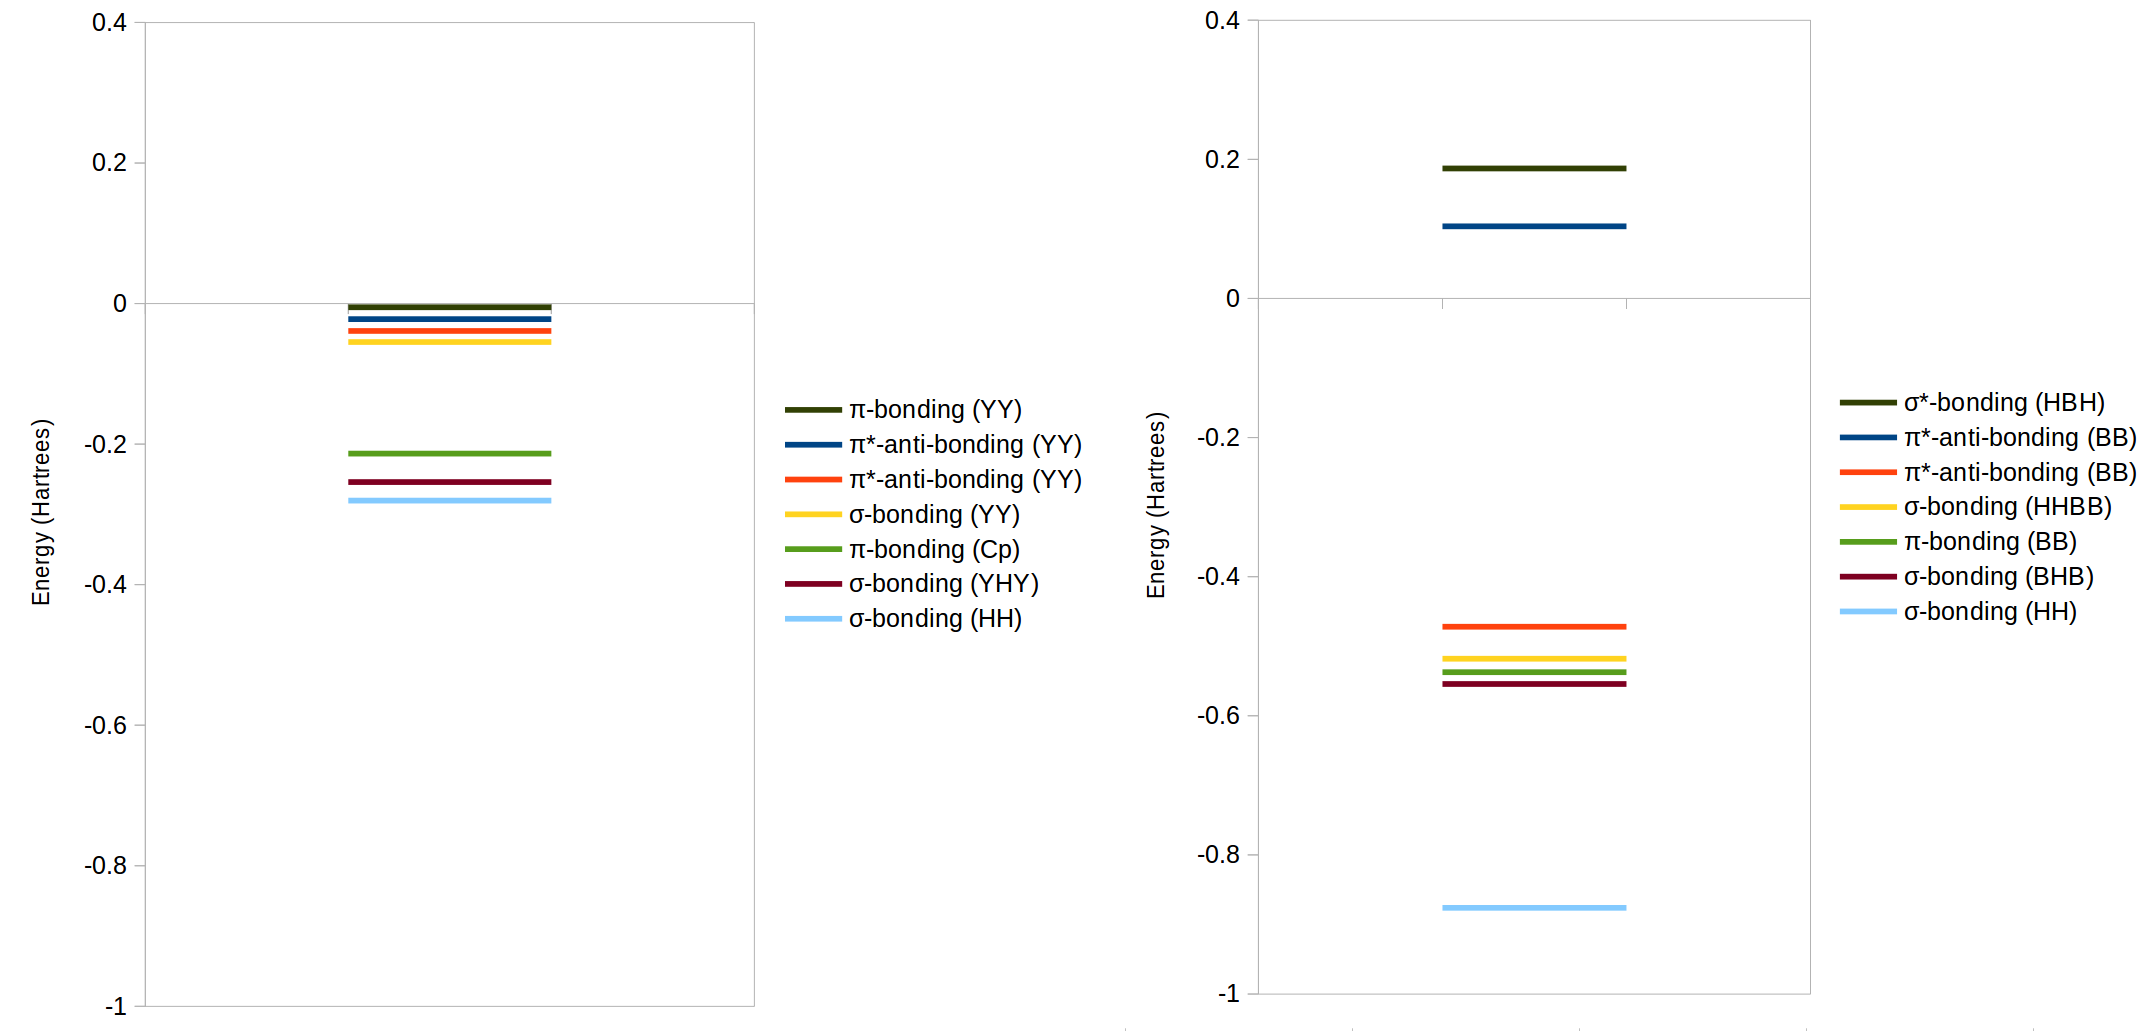
\includegraphics[scale=0.2]{minimal_mos.png}
  \caption{This is a comparison of the minimal molecular orbital model
    of the electronic structure of the neutral Y$\mu$ - H$_2$Y unit and B$\mu$ - H$_2$B
    unit in diborane (cyan and purple). Additional energy levels included for reference.}
  \label{fig:minimal}
\end{figure}

However, the neutral molecule's LUMO is $\sigma$-bonding between
the d-orbitals of the Yttrium metal centers, unlike the LUMO of B$_2$H$_6$
which is $\pi$-antibonding between the Boron atoms.

\begin{figure}[H]
  \centering
  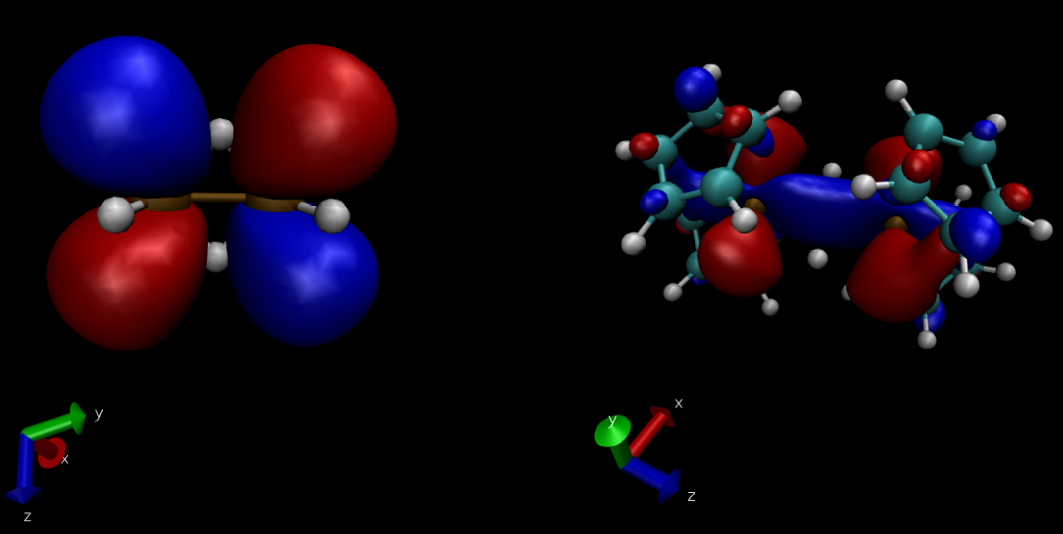
\includegraphics[scale=0.2]{lumo.png}
  \caption{The isosurfaces of pi* antibonding orbital between
the p-orbitals of Boron in diborane (LUMO) (left)
    and direct sigma bonding orbital between the d-orbital yttirum in the neutral bimetallic Yttrium
    complex (LUMO) (right) are shown with a contour value of 0.03.}
  \label{fig:lumo}
\end{figure}

%\comment{insert LUMO of B2H6 and neutral complex here}
%
%This can be used to create a minimal molecular orbital diagram
%for both the neutral molecule and B$_2$H$_6$.(Question 4.1.5)
%
%\begin{figure}[H]
%  \centering
%  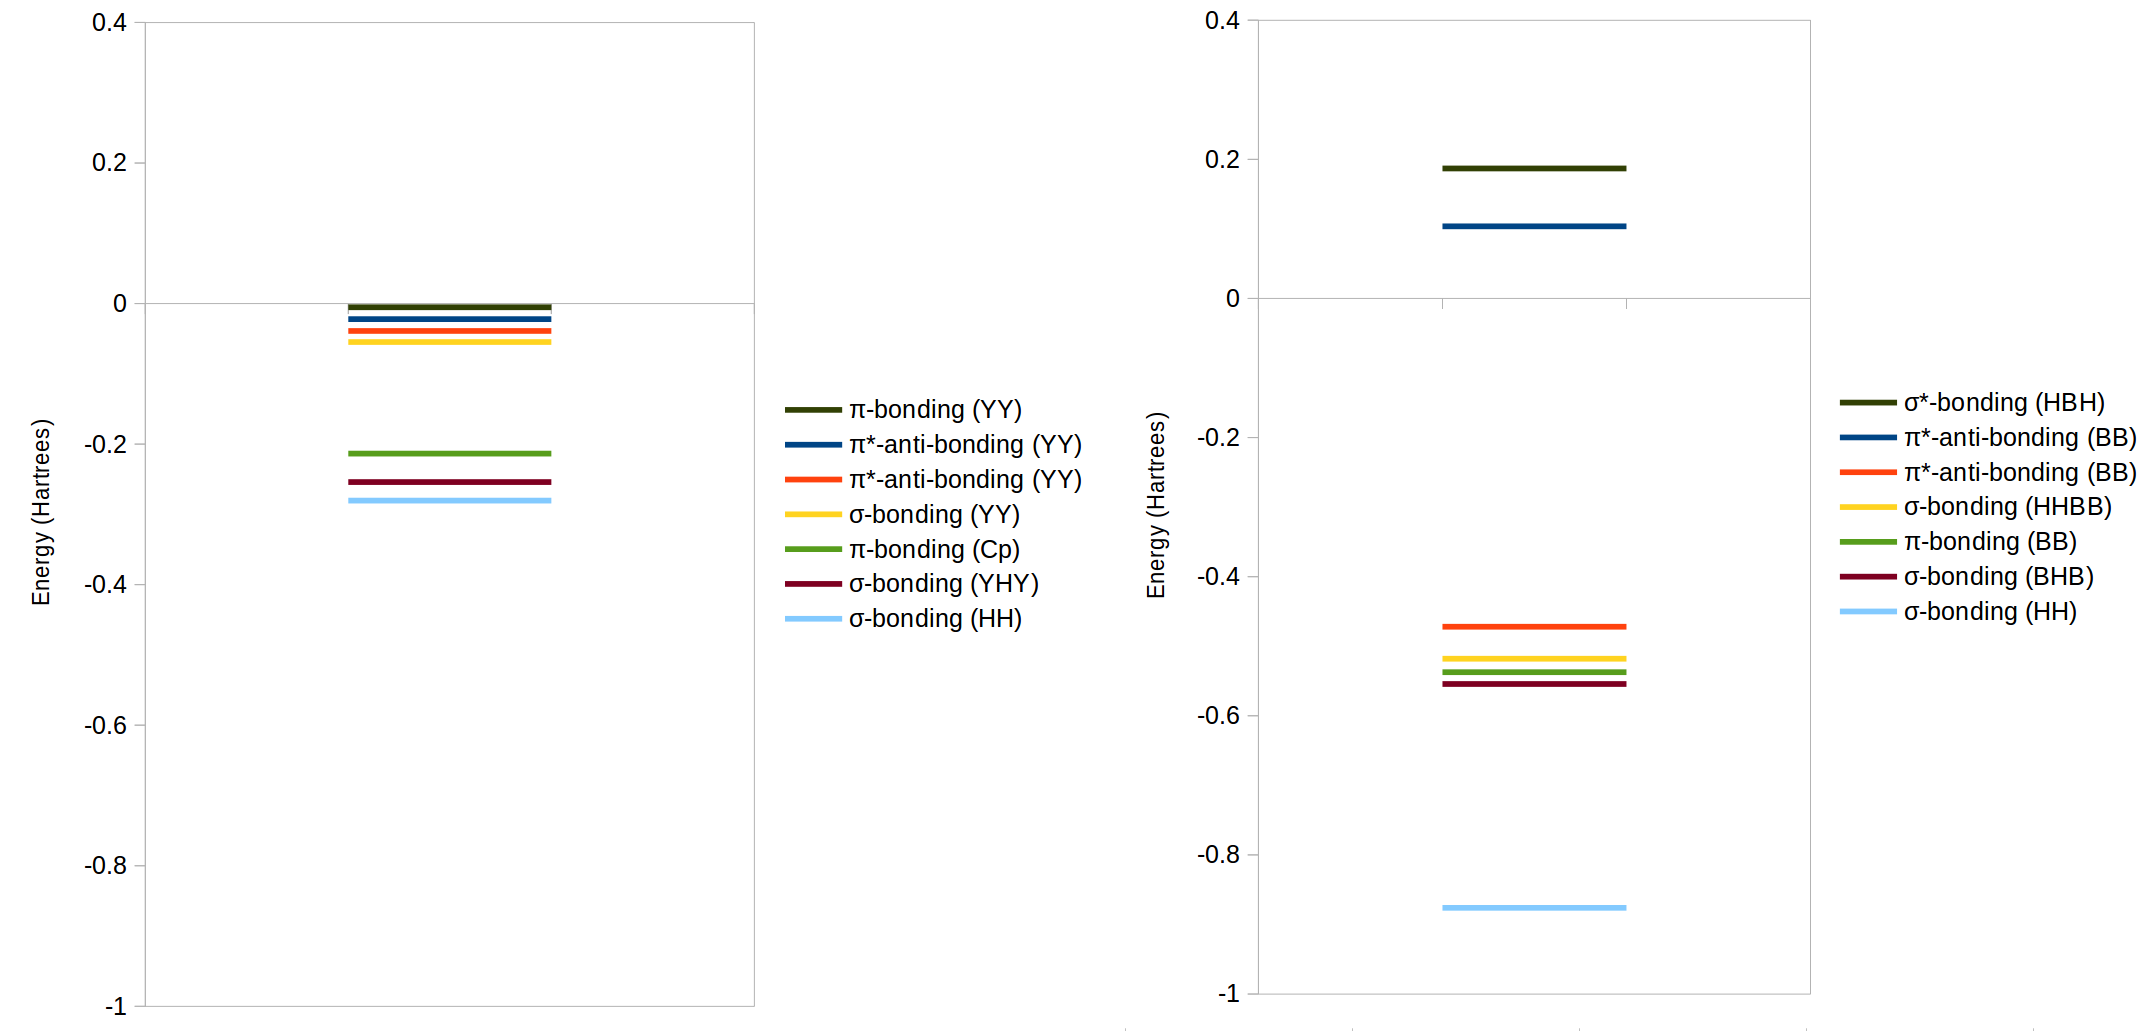
\includegraphics[scale=0.2]{minimal_mos.png}
%  \caption{This is a comparison of the minimal molecular orbital model
%    of the he electronic structure of the Y$\mu$ - H$_2$Y unit and B$\mu$ - H$_2$B
%    unit in diborane with a contour value of 0.03.}
%  \label{fig:minimal}
%\end{figure}
%
%\comment{insert minimal MO here. }

The LUMO of the neutral molecule is half-filled in the anion,
forming the SOMO of the anion. The molecular orbitals for the
anion are visually similar to the neutral Yttrium complex with
the exception of HOMO-9 which is shown below.

\begin{figure}[H]
  \centering
  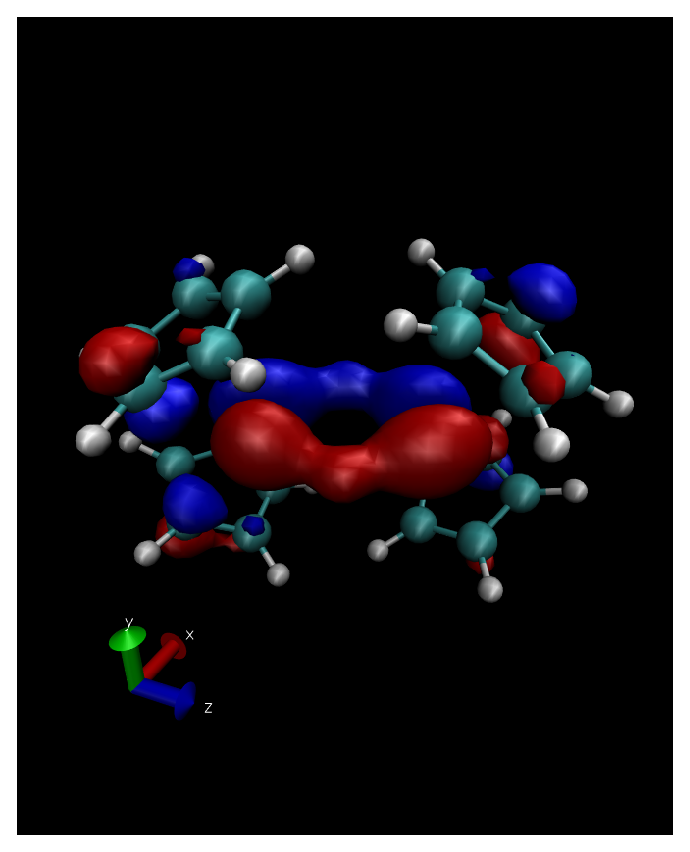
\includegraphics[scale=0.4]{73n.eps}
  \caption{HOMO-9 for the anionic Yttrium metal illustrated by the natural
    molecular orbitals at 0.03 contour value. This orbital is
now sigma bonding between the p-orbital of the Yttrium and the
s-orbital of the hydrides.}
\end{figure}

\begin{figure}[htbp]
  \centering
  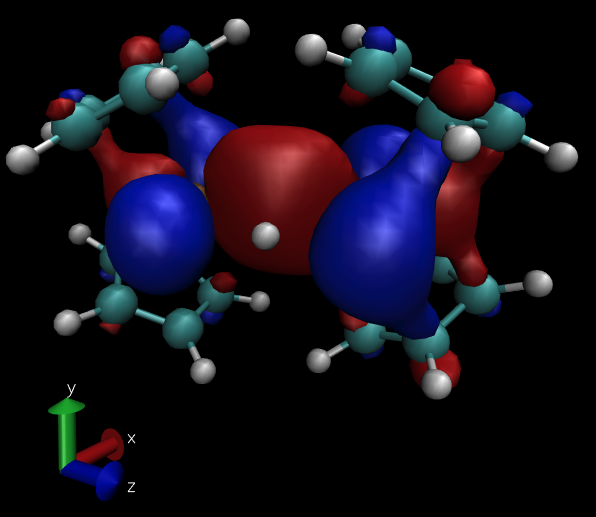
\includegraphics[scale=0.2]{83an.png}
  \caption{This represents the SOMO of the anion bimetallic Yttrium complex.
    It is a $\sigma$ bonding orbital between the d-orbitals of the Yttrium metal
    centers.}
\end{figure}

%\comment{insert SOMO of anion here.}

The SOMO is half-filled therefore there is a bond order of 0.5
between the metal centers in the anion. (Question 4.1.4)
The SOMO appears to have significant contribution from the 3d 
atomic orbitals of Yttrium. The diffuse nature of the 3d
orbitals results in a relatively weaker $\sigma$ bond when
compared to the 2p and 2s orbitals, but there is metal-metal
bonding in the complex. The SOMO has small contributions from the Cp
ligands, but this is probably an artifact due to basis set
incompleteness. B$_2$H$_6$ does not have accessible 3d orbitals,
thus it's anion would display very different chemistry when
compared to this anion.

%The bridging hydride 3-center-2-electron bonds are also verified
%in the anion.

%\comment{insert nmo for anion hydride bonds here.}

\section{Conclusions}

Metal-metal bonding between Yttrium has been analysed for the
neutral molecule and anion. While the neutral molecule does not
have metal-metal bonding in this calculation, reducing the complex
by adding an electron results in a weak metal-metal bond of bond order 0.5.

This is in contrast to published results and can be due to a number of
factors such as the small basis set and not localizing orbitals.

%\section*{Acknowledgments}
%
%This section should acknowledge any additional sources of support from
%professionals who aren't co-authors but helped you complete your work. For
%example, O. H. would like to acknowledge useful discussions with The
%Three Stooges. Often, funding agencies mandate that funding be
%acknowledged in this section. 

\printbibliography

\end{document}
